% !TeX spellcheck = de_DE
\documentclass{alex_gp}

\name{Alexander Helbok}
\course{Grundpraktikum}
\hwnumber{7}
\spacing{}
\usepackage{biblatex}
\usepackage{stackengine}


\begin{document}
\renewcommand{\labelenumi}{\alph{enumi})}


\begin{mybox}{RC Entladung}
	\begin{wrapfigure}[16]{r}{4.25cm}
		\vspace{-0.5cm}
		\begin{circuitikz}[european]
			\draw (0,0)-- (0,4)
			to[R, l_=$10 \unit{\ko}$, name=R] (4,4)   -- (4,2.5)
			to[rmeter, t=$U_1$] (4,1.5)	--	(4,0)
			to[opening switch, mirror] (2,0) -- (2,0)
			to[thick, battery1, a=\smash{\stackunder[6pt]{\( 3.3 \unit{V} \)}{$_-$~~~$_+$}}](0, 0);
%			
			\draw (0,0)	--	(0,2)
			to[thick, C, l=$C$] (3.6, 2);

			\node  at (R.center) {$R$};
		\end{circuitikz}
		\caption{RC Schaltkreis mit einem Widerstand  \(  R = 10.0(1) \unit{\ko} \) und einem Kondensator \( C = 2.2 \unit{\micro\farad} \). An einer Stelle wird mit einem analogen Port die Spannung gemessen.}
		\label{fig:1}
	\end{wrapfigure}
	\noindent
	Kondensatoren sind elektronische Bauteile, die bei vorhandener Spannung sich aufladen und Ladungen speichern. Unterbricht man dann den Stromfluss, entlädt sich der Kondensator. Um dieses Verhalten zu untersuchen, wurde ein Schaltkreis gebaut (Siehe \autoref{fig:1}) mit einem Widerstand \( R = 10.0(1) \unit{\ko} \) und Kondensator \( C = 2.2 \unit{\micro\farad} \). Der Kondensator wird als ideal angenommen, da die Toleranz nicht angegeben war. 
	
	Der Versuch wird mit geschlossenem Schalter gestartet und es wird ein paar Sekunden gewartet bis sich der Kondensator zur Gänze aufgeladen hat. Dann wird der Schalter geöffnet (in diesem Fall wurde ein Kabel ein- und ausgesteckt), wodurch sich der Kondensator entlädt. Während des ganzen Vorganges wird an \( U_1 \) die Spannung gemessen. 
	
	Um die Unsicherheit der Spannungsmessung abzuschätzen, wurde mit zwei Widerständen ein einfacher Spannungsteiler gebaut und für \( 5 \unit{s} \) die Spannung gemessen. Der Fehler der analogen Sensoren wird in den folgenden Versuchen auf die Standardabweichung \( \sigma = 1.85 \unit{mV} \) dieser Messung gesetzt. 
	
	Die Spannung am Kondensator wird laut Skript durch 
	\begin{equation}\label{eqn:tau}
		V(t) = V(0)\expo[-][t/RC] = V(0)\expo[-][t/\tau]
	\end{equation}
	beschrieben, wobei \( \tau = RC \) gesetzt wurde. Die Spannung wird also durch eine exponentielle Zerfallskurve beschrieben mit Zerfallsparameter \(  \tau \). 
	
	In \autoref{fig:ExpFit} ist die Spannung während der Entladung des Kondensators auf die Zeit aufgetragen. Die Fehlerbalken wurden nicht eingezeichnet, da man sie nicht ausmachen könnte. Die Spannung zu Beginn der Entladung beträgt \(  3 \unit{V} \) (Sättigungsgrenze des ADC) und pendelt sich gegen Ende bei \( 0.00073 \unit{V} \) ein. Da wir diese beiden Randbedingungen kennen, wurde eine Funktion der Form \( f(x) = 3\expo[-][x/b] + 0.00073 \) an die Daten angepasst. Dadurch haben wir die drei Freiheitsgrade eines allgemeinen exponentiellen Fits auf einen reduziert. Für den Fit wurden 10 ungefähr gleichmäßig verteilten Datenpunkte herangezogen. Die Fitfunktion, der Fitparameter b und die ausgewählten Messpunkte sind in \autoref{fig:ExpFit} in rot dargestellt.
 	
	\begin{figure}[H]	
		\centering
		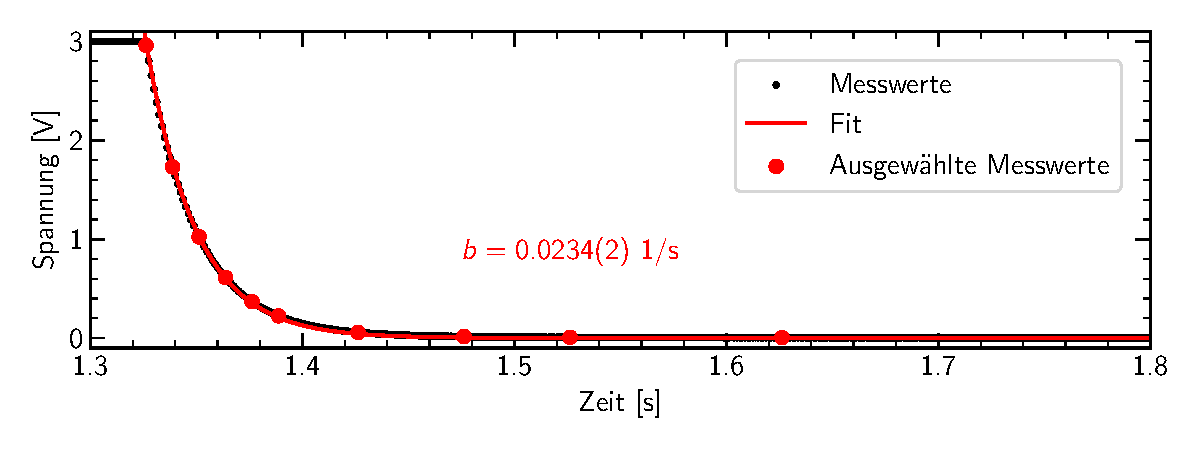
\includegraphics[width=\textwidth]{Versuch7_1}
		\caption{Zeitliche Spannungsdaten während der Kondensatorentladung. In rot wurde die exponentielle Fitfunktion aufgetragen. Die für den Fit herangezogenen Datenpunkte sind ebenfalls rot hervorgehoben. Der Fehler der Spannungsdaten wird nicht dargestellt, dar dieser zu klein.}
		\label{fig:ExpFit}
	\end{figure}

	Die Fitfunktion wurde so gewählt, dass \( \tau_{\text{exp}} = b = 0.0234(2) \unit{1/s} \) gilt und daher Wert und Unsicherheit von Tau direkt vom Fitprogramm berechnet wird. Verwendet man \( \tau = RC \) und die Werte für 
	erhält man \( \tau_{\text{theo}} = 0.0220(2) \unit{1/s} \). Die Unsicherheit hier kommt nur aus dem Widerstand, da der Kondensator als ideal angenommen wird. Letzteres ist aber normalerweise nicht der Fall, wodurch wahrscheinlich die Diskrepanz zwischen experimentell und theoretisch bestimmten Wert für die Zeitkonstante \( \tau \) rührt.
\end{mybox}

\begin{mybox}{RC Frequenzanalyse}
	\begin{wrapfigure}[19]{r}{4.25cm}
		\vspace{-0.5cm}
		\begin{circuitikz}[european]
			\draw (2.6,0) -- (2,0)
			to[line width=0.3pt, rmeter, t=$U_1$] (0,0)
			to[R, l_=$10 \unit{\ko}$, name=R] (0,4)
			to[rmeter, t=$U_2$] (4,4)
			to[thick, C, l_=$C$] (4,0) -- (3.4,0);
			
			\draw (3,-0.4) to[sV] (3, 0.4);
			
			\draw[latex-, line width=0.5pt] (2.7,0.65) -- (3.3, 0.65);
			
			\node  at (R.center) {$R$};
		\end{circuitikz}
		\caption{RC Schaltkreis mit einem Widerstand  \(  R = 10.0(1) \unit{\ko} \) und einem Kondensator \( C = 2.2 \unit{\micro\farad} \) der an einer Wechselstromspannungsquelle angeschlossen ist. An zwei Stellen wird über einen analogen Port die Spannung aufgezeichnet.}
		\label{fig:2}
	\end{wrapfigure}
	Legt man Wechselstrom an einem Kondensator an, werden Phase und Amplitude der Schwingung verändert, wobei das von der Frequenz der Spannung und den Eigenschaften der elektronischen Komponenten abhängt. Um dieses Verhalten zu untersuchen, wurde ein Schaltkreis mit einem Widerstand  \(  R = 10.0(1) \unit{\ko} \) und einem Kondensator \( C = 2.2 \unit{\micro\farad} \) aufgebaut (Siehe \autoref{fig:2}). Als Wechselstromspannungsquelle wurde mit einem Laptop über ein AUX-Kabel ein Sinusförmiges Signal eingespielt.  
	
	An \( U_1 \) wird die eingespielte Spannung als Referenzmessung aufgezeichnet, während an \( U_2 \) die veränderte Spannung Spannung gemessen wird. Es wurde für Frequenzen \( f = 1, 3, 7, 10, 20 \unit{Hz} \) für 5 Sekunden Daten aufgezeichnet. Unter der Annahme, dass die Frequenz perfekt ist, kennt man auch die Periode \( T = 1/f \) genau und man kann die Schwingungsdaten falten (da das Signal periodisch ist). Sprich man wendet den modulo Operator auf die Daten an und legt \( T-\)sekunden lange Zeitintervalle übereinander (und normiert diese neue Einheitslose Zeitachse von 0 bis 1).
	
	Ob die Faltung erfolgreich war erkennt man daran, dass die Daten bis auf wenige Ausreißer eine schöne Kurve beschreiben. In \autoref{fig:SineFit} sieht man die gefalteten Daten für \( f = 7 \unit{Hz} \) und ohne die Güte zu quantifizieren (zb. mittels shortest string) würde ich behaupten, dass die Faltung passt. Diese Darstellung hat viele Vorteile, in unserem Fall ermöglicht sie den Fit einer Sinusfunktion der Form \( f(x) = A*\sin(\omega x + \phi) \) auf ein langes Zeitintervall, auch wenn die Daten nur Stückweise eine Sinusfunktion beschreiben (da negative Spannungen nicht aufgezeichnet werden). 
	
	\begin{figure}[H]	
		\centering
		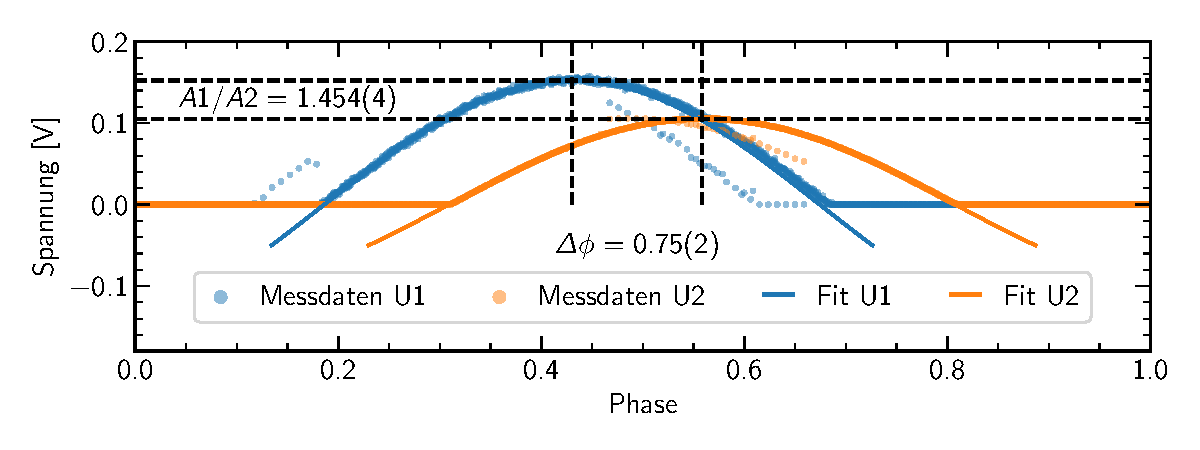
\includegraphics[width=\textwidth]{Versuch7_2}
		\caption{Zeitliche Spannungsdaten während der Kondensatorentladung. In rot wurde die exponentielle Fitfunktion aufgetragen. Die für den Fit herangezogenen Datenpunkte sind ebenfalls rot hervorgehoben. Der Fehler der Spannungsdaten wird nicht dargestellt, dar dieser zu klein.}
		\label{fig:SineFit}
	\end{figure}
	
	
	\begin{center}
		\captionof{table}{Gemessenes Amplitudenverhältnis \( A_1/A_2 \) und Phasenverschiebung \( \Delta\phi \) für verschiedene Frequenzen. Dazu die draus errechneten Werte für \( \tau \).}
		\begin{tabular}{@{\extracolsep{5mm}} 
				r
				S[table-format=1.4(2)]
				S[table-format=1.4(2)]
				S[table-format=1.4(2)]
				S[table-format=1.4(2)]
				S[table-format=1.4(2)]
			}
			\toprule
			\makecell[t]{}
			&   {\makecell[t]{\( 1 \unit{Hz} \)}}
			&   {\makecell[t]{\( 3 \unit{Hz} \)}}
			&   {\makecell[t]{\( 7 \unit{Hz} \)}}
			&   {\makecell[t]{\( 10 \unit{Hz} \)}}
			&   {\makecell[t]{\( 20 \unit{Hz} \)}} \\
			\midrule
			\( A_1/A_2 \) & 1.016(2) & 1.101(2) & 1.454(4) & 1.788(5) & 3.095(15) \\
			\( \tau_{A}\ [1/\text{s}]\) & 0.029(2) & 0.0244(3) & 0.02400(11) & 0.02359(10) & 0.02331(13) \\
			\( \Delta\phi \) & 0.140(11) & 0.483(13) & 0.75(2) & 1.00(2) & 1.29(4) \\
			\( \tau_{\phi}\ [1/\text{s}]\) & 0.022(2) & 0.0278(8) & 0.0211(7) & 0.0247(12) & 0.028(5) \\
			\bottomrule
		\end{tabular}
		\label{table:1}
	\end{center}


	\begin{align}\label{eqn:tauq}
		\abs{\frac{A_1}{A_2}}^2 = 1 + (\omega\tau_A)^2 &\quad \Longleftrightarrow\quad \tau_A = \frac{\SQRT{\abs{\tfrac{A_1}{A_2}}^2 - 1}}{2\pi f}\\
		\tan(\Delta\phi) = -\omega\tau_{\phi} &\quad \Longleftrightarrow\quad \tau_{\phi} = -\frac{\tan(\Delta\phi)}{2\pi f}
	\end{align}
\end{mybox}

\begin{mybox}{RLC Schwingkreis}
	So wie Kondensatoren, verändern Induktoren die Phase und Amplitude der Schwingung. Der U
\end{mybox}


\end{document}